\emph{Temporal-difference learning} is a combination of \myref{ch:mcm}{MC}
and \myref{ch:dp}{DP} methods, it generates experience from which it learns, like \emph{MC},
and it bootstraps like \emph{DP}.

\section{TD Prediction}
\label{sec:td_prediction}
Similar to how \emph{MC} methdods predict but we stop right after the first step and then
use the approximated value.
Basically, the target is $R_{t+1}+\gamma V(S_{t+1})$ instead of $G_t$.

\begin{myequation}{6.2}
    V(S_t)\leftarrow V(S_t) + \alpha\left[R_{t+1}+\gamma V(S_{t+1})-V(S_t)\right]
\end{myequation}

This is called $TD(0)$ or \emph{one-step TD}\label{t:tdl-one_step_td}.

\begin{center}
    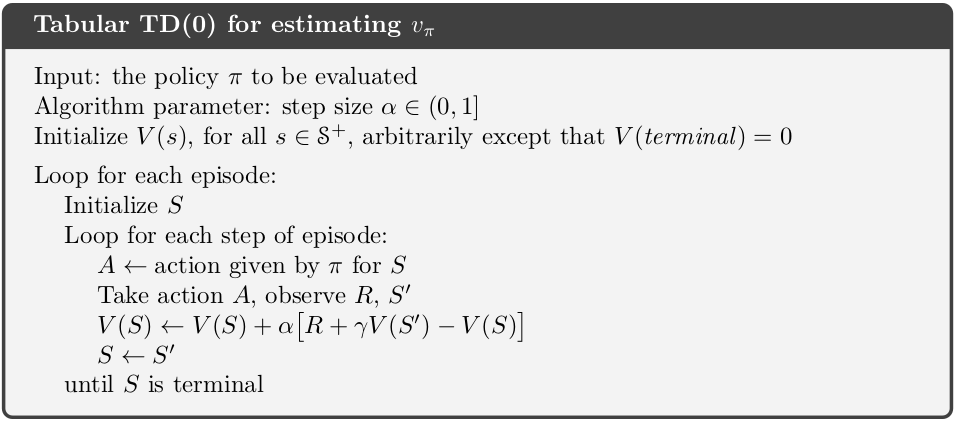
\includegraphics[width=\textwidth]{img/td0.png}
\end{center}

We can notice that the value in the brackets in (\ref{eq:6.2}) is a sort of error.
That error is called \emph{TD error} ($\delta$)\label{t:td_error} and it is the
difference from the estimated value of $S_t$ and the better estimate after the next step
$R_{t+1}+\gamma V(S_{t+1})$.

\begin{myequation}{6.5}
    \delta_t\doteq R_{t+1}+\gamma V(S_{t+1})-V(S_t)
\end{myequation}

\section{Advantages of TD Prediction Methods}
\label{sec:advantages_of_td_prediction_methods}

\section{Optimality of TD(0)}
\label{sec:optimality_of_td0}
Consider an example where we use \emph{batch updating}.
\myref{ch:temporal_difference_learning}{TD(0)} and constant $\alpha$ \myref{ch:mcm}{MCM}
converge to different values.
Observe the following episodes:
\begin{wrapfigure}{r}{0.4\linewidth}
    \centering
    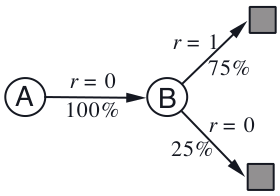
\includegraphics[scale=0.4]{img/ex6_4.png}
\end{wrapfigure}
\begin{multicols}{2}
    \begin{enumerate}
        \item $A,0,B,0$
        \item $B,1$
        \item $B,1$
        \item $B,1$
        \item $B,1$
        \item $B,1$
        \item $B,1$
        \item $B,0$
    \end{enumerate}
\end{multicols}

Both batch TD(0) and batch MC would conclude that $V(B)=\frac{3}{4}$ but TD(0) would
approximate $V(A)=V(B)=\frac{3}{4}$ whereas MC would approximate $V(A)=0$ because the one
episode we go through the state we get reward $0$.

Batch MC methods always find the estimates that minimize mean-squared error on the
training set, whereas batch TD(0) always finds the estimates that would be exactly correct
for the maximum-likelihood model of the Markov process.
In general, the \emph{maximum-likelihood estimate} of a parameter is the parameter value
whose probability of generating the data is greatest.
In this case, the maximum-likelihood estimate is the model of the Markov process formed in the
obvious way from the observed episodes: the estimated transition probability from $i$ to $j$
is the fraction of observed transitions from $i$ that went to $j$, and the associated expected
reward is the average of the rewards observed on those transitions.
Given this model, we can compute the estimate of the value function that would be exactly
correct if the model were exactly correct.
This is called the \emph{certainty-equivalence estimate} because it is equivalent to assuming
that the estimate of the underlying process was known with certainty rather than being
approximated.

\section{Sarsa: On-policy TD Control}
\label{sec:sarsa_on_policy_td_control}
Instead of state values we use action values:
\begin{myequation}{6.7}
    \delta_t\doteq R_{t+1}+\gamma Q(S_{t+1},A_{t+1})-Q(S_t,A_t) \\
    Q(S_t,A_t)\leftarrow Q(S_t,A_t)+\alpha\cdot\delta_t
\end{myequation}

\begin{center}
    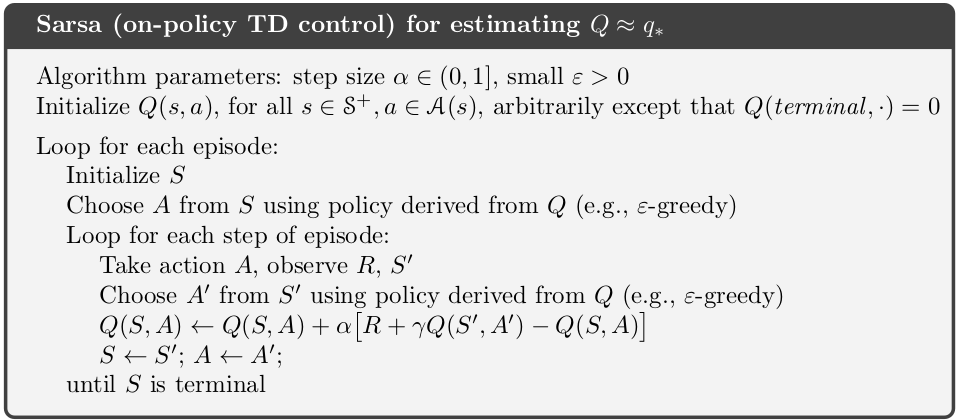
\includegraphics[width=\textwidth]{img/alg_sarsa.png}
\end{center}

\section{Q-Learning: Off-policy TD Control}
\label{sec:q_learning_off_policy_td_control}
Instead of using $Q(S_{t+1}, A{t+1})$ for action $A_{t+1}$ taken by the \emph{behavior policy} we
use $\max_aQ(S_{t+1}, a)$.

\begin{myequation}{6.8}
    \delta_t\doteq R_{t+1}+\max_aQ(S_{t+1},a)-Q(S_t,A_t) \\
    Q(S_t,A_t)\leftarrow Q(S_t,A_t)+\alpha\cdot\delta_t
\end{myequation}

All that is required for correct convergence is that all pairs continue to be updated.

\begin{center}
    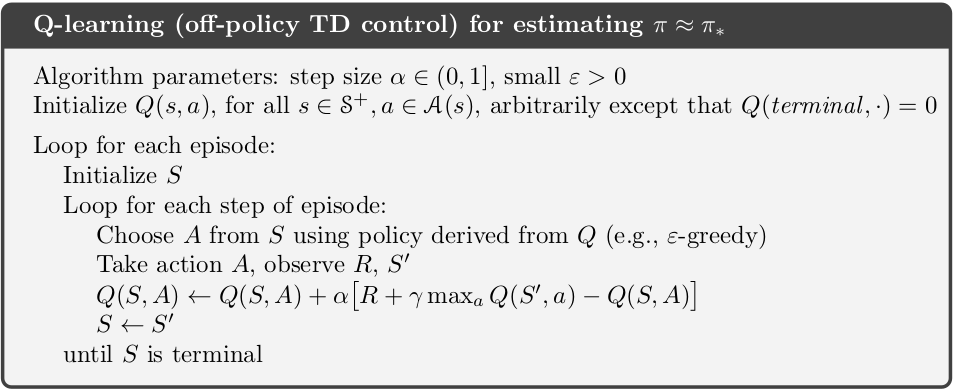
\includegraphics[width=\textwidth]{img/alg_q_learning.png}
\end{center}

\section{Expected SARSA}
\label{sec:expected_sarsa}

\begin{myequation}{6.9}
    \begin{aligned}
        \delta_t
        &\doteq R_{t+1}+\gamma\mathbb{E}\left[Q(S_{t+1},A_{t+1}\mid S_{t+1})\right]-Q(S_t,A_t)\\
        &\doteq R_{t+1}+\gamma\sum_a\pi(a\mid S_{t+1})Q(S_{t+1},a)-Q(S_t,A_t)
    \end{aligned} \\
    Q(S_t,A_t)\leftarrow Q(S_t,A_t)+\alpha\cdot\delta_t
\end{myequation}

\section{Maximization Bias and Double Learning}
\label{sec:maximization_bias_and_double_learning}
A maximum over estimated values is used implicitly as an estimate of the maximum value, which can
lead to a significant positive bias.
To see why, consider a single state s where there are many actions a whose true values,
$q(s,a)$, are all zero but whose estimated values, $Q(s,a)$, are uncertain and thus distributed
some above and some below zero.
The maximum of the true values is zero, but the maximum of the estimates
is positive, a positive bias.
We call this \emph{maximization bias}\label{t:maximization_bias}.

The reason this bias occurs is because we are using the same state-action value function to
approximate $q(s,a)$ and then using the maximum of the estimation of $q(s,a)$ to estimate the
maximum of $q(s,a)$ - the optimal action.
To attempt and mitigate this issue, we can learn two independent estimates of the state-action
value ($Q_1, Q_2$) and then using them generate an unbiased estimate of the maximum of $q(s,a)$.
We get the optimal action from one of the estimates to update the other.
\begin{myequation}{6.10}
    \delta_t\doteq R_{t+1}+\gamma Q_1(S_t,\argmax_aQ_2(S_{t+1},a))-Q_1(S_t,A_t) \\
    Q_1(S_t,A_t)\leftarrow Q_1(S_t,A_t)+\alpha\delta_t
\end{myequation}

\begin{center}
    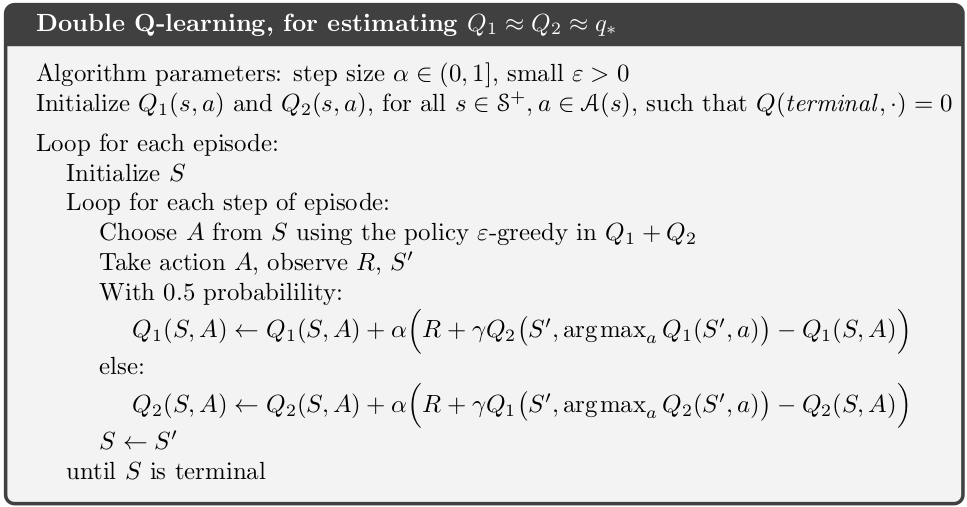
\includegraphics[width=\textwidth]{img/alg_dq_learning.png}
\end{center}

\section{Games, Afterstates, and Other Special Cases}
\label{sec:games_afterstates_and_other_special_cases}
A conventional state-value function evaluates states in which the agent has the option of
selecting an action, but the state-value function used in tic-tac-toe evaluates board positions
after the agent has made its move.
Let us call these \emph{afterstates}\label{t:afterstate}, and value functions over these,
\emph{afterstate value functions}\label{t:afterstate_value_functions}.

\begin{figure}[h]
    \centering
    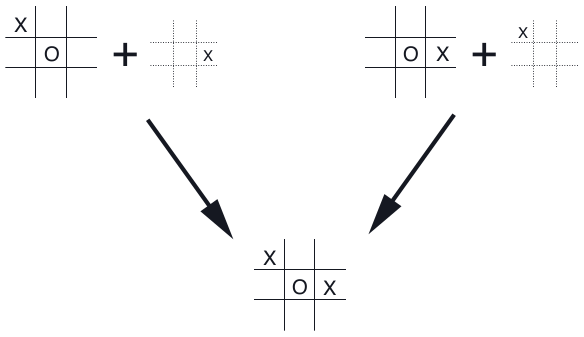
\includegraphics[width=0.8\textwidth]{img/afterstate_example.png}
    \caption{Two different state-action pairs that result in the same afterstate and therefore
        should have the same $Q$.}
    \label{fig:afterstate_example}
\end{figure}

A conventional action-value function would have to separately assess both pairs, whereas an
afterstate value function would immediately assess both equally.

\section{Summary}
In this chapter we introduced a new kind of learning method, temporal-difference (TD)
learning, and showed how it can be applied to the reinforcement learning problem.
As usual, we divided the overall problem into a prediction problem and a control problem.
TD methods are alternatives to Monte Carlo methods for solving the prediction problem.
In both cases, the extension to the control problem is via the idea of \myref{sec:gpi}{GPI}
that we abstracted from dynamic programming.
This is the idea that approximate policy and value functions should interact in such a way that
they both move toward their optimal values.
One of the two processes making up \myref{sec:gpi}{GPI}  drives the value function to accurately
predict returns for the current policy; this is the prediction problem.
The other process drives the policy to improve locally (e.g., to be $\epsilon$-greedy) with
respect to the current value function.
When the first process is based on experience, a complication arises concerning
maintaining sufficient exploration.
We can classify TD control methods according to whether they deal with this complication by
using an on-policy or off-policy approach.
\myref{sec:sarsa_on_policy_td_control}{Sarsa} is an on-policy method, and
\myref{sec:q_learning_off_policy_td_control}{Q-learning} is an off-policy method.
\myref{sec:expected_sarsa}{Expected Sarsa} is also an off-policy method as we present it here.
There is a third way in which TD methods can be extended to control which we did not include in
this chapter, called actor–critic methods.
These methods are covered in full in Chapter 13.
The methods presented in this chapter are today the most widely used reinforcement
learning methods.
This is probably due to their great simplicity: they can be applied online, with a minimal amount
of computation, to experience generated from interaction with an environment; they can be expressed
nearly completely by single equations that can be implemented with small computer programs.
In the next few chapters we extend these algorithms, making them slightly more complicated and
significantly more powerful.
All the new algorithms will retain the essence of those introduced here: they will be able
to process experience online, with relatively little computation, and they will be driven
by TD errors.
The special cases of TD methods introduced in the present chapter should rightly be called
one-step, tabular, model-free TD methods.
In the next two chapters we extend them to n-step forms (a link to Monte Carlo methods) and forms
that include a model of the environment (a link to planning and dynamic programming).
Then, in the second part of the book we extend them to various forms of function approximation
rather than tables (a link to deep learning and artificial neural networks).
Finally, in this chapter we have discussed TD methods entirely within the context of
reinforcement learning problems, but TD methods are actually more general than this.
They are general methods for learning to make long-term predictions about dynamical systems.
For example, TD methods may be relevant to predicting financial data, life spans, election outcomes,
weather patterns, animal behavior, demands on power stations, or customer purchases.
It was only when TD methods were analyzed as pure prediction methods, independent of their use in
reinforcement learning, that their theoretical properties first came to be well understood.
Even so, these other potential applications of TD learning methods have not yet been extensively
explored.
